\documentclass[12pt]{article}
\usepackage[utf8x]{inputenc}
\usepackage{amsmath}
\usepackage{multicol}
\usepackage{graphicx}
\usepackage{float}
\usepackage{dsfont}
\usepackage{textcomp}
\usepackage{multirow}
\usepackage{amsfonts}
\usepackage{hyperref}
\usepackage{cleveref}
\usepackage{fancyhdr}
\setlength{\headheight}{14.5pt}
\renewcommand{\sectionmark}[1]{\markright{#1}{}}
\usepackage[T1]{fontenc}
\usepackage[colorinlistoftodos]{todonotes}
\usepackage[margin=2cm,a4paper]{geometry}
\newgeometry{left=2.0cm,right=2.0cm,top=2.5cm,bottom=2.5cm}
\usepackage{listings}
\setlength{\marginparwidth}{2cm}
\setlength{\parindent}{0pt}
\newcommand{\deriv}{\mathrm{d}}
\lstset{
    language=R,
    basicstyle=\scriptsize\ttfamily,
    commentstyle=\ttfamily\color{red},
    numbers=left,
    numberstyle=\ttfamily\color{blue}\footnotesize,
    stepnumber=1,
    numbersep=5pt,
    backgroundcolor=\color{white},
    showspaces=false,
    showstringspaces=false,
    showtabs=false,
    frame=single,
    tabsize=2,
    captionpos=b,
    breaklines=true,
    breakatwhitespace=false,
    title=\lstname,
    escapeinside={},
    keywordstyle={},
    morekeywords={}
    }
\title{}
\pagestyle{fancy}
\fancyhf{}
\lhead{How has the design of aircraft evolved to avoid radar detection}
\lfoot{PH608: The Sun, The Earth and Mars}
\rfoot{Page \thepage}
\renewcommand{\headrulewidth}{1pt}
\renewcommand{\footrulewidth}{1pt}
\begin{document}
\begin{titlepage}
\newgeometry{left=1.0in,right=1.0in,top=2.0in,bottom=2.0in}
\newcommand{\HRule}{\rule{\linewidth}{0.5mm}}
\begin{centering} 
%---------------------------------------------------------------------------
%	HEADING SECTIONS
%---------------------------------------------------------------------------

\includegraphics[scale=0.7]{Images/Uni_of_Kent.png}\\[1cm]
%---------------------------------------------------------------------------
%	TITLE SECTION
%---------------------------------------------------------------------------
\HRule \\ [0.3cm]
\Huge{\bfseries{How has the design of aircraft \\ evolved to avoid radar detection}} \\
\textsc{\large PH608: The Sun, The Earth and Mars}\\ [-0.1cm]
\textsc{\large Astronomy, Space Science and Astrophysics}\\ [-0.2cm]
\HRule \\[0.5cm]
%---------------------------------------------------------------------------
%	AUTHOR SECTION
%---------------------------------------------------------------------------
\begin{minipage}{0.625\textwidth}
\begin{center} \large
{\large Date: 27th November 2020}\\[0.2cm]
{\large Report Author: Lukasz R Tomaszewski}\\[0.2cm]
{\large Word Count: 1568}\\
\end{center}
\end{minipage}\\[2cm]
\vfill
\end{centering} 
\end{titlepage}
%---------------------------------------------------------------------------
\newpage
\begin{titlepage}
\begin{tableofcontents}
\end{tableofcontents}
\end{titlepage}
\newpage
%---------------------------------------------------------------------------
%	INTRODUCTION
%---------------------------------------------------------------------------
\section{Introduction}
\label{Introduction Section}

Since its birth in the late 1800s, it was only until the late 1930s did radar detection see major attention as it was developed to search and detect flying aircraft. Since this, the last century has shown significant improvement not only in radar detection but aircraft design as well, the evolution of aircraft design mainly started out to create fast fighter aircraft and then later turned into radar avoidance. The development of advanced RADAR was engineered before aircraft were able to be developed to avoid them, this mainly in the military was important and millions of dollars went into aircraft evolution with the prime goal of avoid such advanced RADAR technology. The Doppler shift effect played a key role in the development of RADAR systems in which the change in the waves frequency when in contact with an aircraft allowed said aircraft to be detected and its speed and direction to be analysed. The evolution of such aircraft saw a complete remodel of the structure of the aircraft, the materials used and other physical abilities that either impede RADAR detection or subdue the radio waves by either absorbing, refracting or reducing the refraction/ reflection of the radio signals. This evolution of aircraft would see the birth of stealth aircraft and a new type of aircraft warfare to begin and the development of other technology such as autonomous aircraft and navigation. \\

%---------------------------------------------------------------------------
%	HISTORY
%---------------------------------------------------------------------------
\section{History of Radar and basic aircraft evolution}
\label{History Section}

In the 1880s Heinrich Hertz proves the existence of radio and electromagnetic waves by experimenting with Maxwell's theory of electromagnetic radiation. This ultimately allowed Christian Hülsmejer in 1904 to create and patent the Telemobiloscope, a rudimentary radar (radio detection and ranging) device that could detect objects at a distance but could not calculate said distance \cite{Lecture1}. Though World War 1 followed and aircraft design had improved drastically since Wilbur and Orville Wright invented the first aircraft in 1903, at the star to the war the design of aircraft focused on manoeuvrability and speed for high altitude dog fights and bombing runs. Throughout the war aircraft were used for surveillance by taking aerial images of enemy positions and supplies, the Germans first developed a form of visual stealth aircraft by using light coloured paint and a transparent fuselage, this would be the first example of how aircraft evolved to avoid detection \cite{Ency}. \\

After World War 1 aircraft design and radar technology improved drastically however throughout World War 2 the latter would prove to have the advantage. With radar technology able detect aircraft miles away and act as an early warning system to allow time for a military counter attack, this ultimately allowed led to the allied victory of the Battle of Britain. The 'Chain Home' system consisted of multiple transmitter and receiver towers along the southern English coast line, the sheer number of these towers allowed for a curtain array to be produced where the entirety of the English channel was constantly scanned and observed for Axis aircraft \cite{Britain}. After the World War 2 radar technology saw severe interest as multiple types of radar were introduced for different sectors including military, aviation, weather, mapping and astronomical usage. \\

RADAR saw both improvements to the its range and the use of the Doppler shift effect became highly effective as the materials used in aircraft changed,its ability to analyse the collected data to produce speed and direction. RADAR would see the technology not only become more powerful but smaller in physical size as allowing it to be placed inside ships, submarines and aircraft allowing for multiple uses and covering greater areas making aircraft detection stronger, this would be seen in the Cold War as not only was RADAR used to detect aircraft but ships, submarines, objects on land and rockets/ missiles. Such advancement led to the discovery of LIDAR (Light Imaging Detection and Ranging) in which a pulsed laser is fired to obtain a distance/ range of an object.

%---------------------------------------------------------------------------
%	RADAR
%---------------------------------------------------------------------------
\section{How does Radar work}
\label{How does Section}

The general type of RADAR (RAdio Detection and Ranging) works by transmitting out electromagnetic waves, when they encounter an aircraft the waves reflect off the aircraft back to the receiver where the data is transmitted as a aircraft and processes the received data to give the speed and direction of the aircraft. In most instances RADAR receiver will be with the transmitter but can also be separate from the transmitter, as shown in \cref{Radardiagram}. 

\begin{figure}[H]
\centering
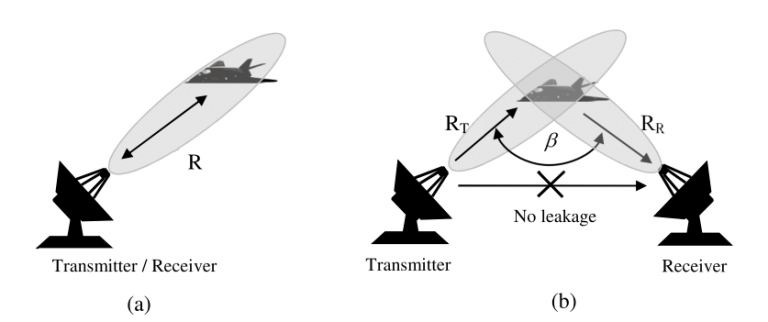
\includegraphics[scale=0.6]{Images/Radar-Systems-a-Monostatic-Radar-b-Bistatic-Radar.png}
\caption{Figure (a) depicts the monostsatic radar method, figure (b) shows the bistatic radar method. Both figures show the path of the outgoing and incoming signals. Source \cite{RadarImage1}}
\label{Radardiagram}
\end{figure}

It's also important to add that RADAR is used on modern aircraft to aid in military targeting systems, automatic drone control and automatic navigation systems. These all use small RADAR system attached to the aircraft and utilise the same principle, the use of radio and electromagnetic waves allowed the Doppler shift effect to help in aircraft detection depicted in \cref{Doppler} where the specific frequency of radio wave is sent out and the once comes into contact with an object will reflect off the object and depending on the objects material density and shape will change the frequency and that altered frequency is picked up by an receiver that changes the new frequency into data that shows an estimated direction and speed of the object.

\begin{figure}[H]
\centering
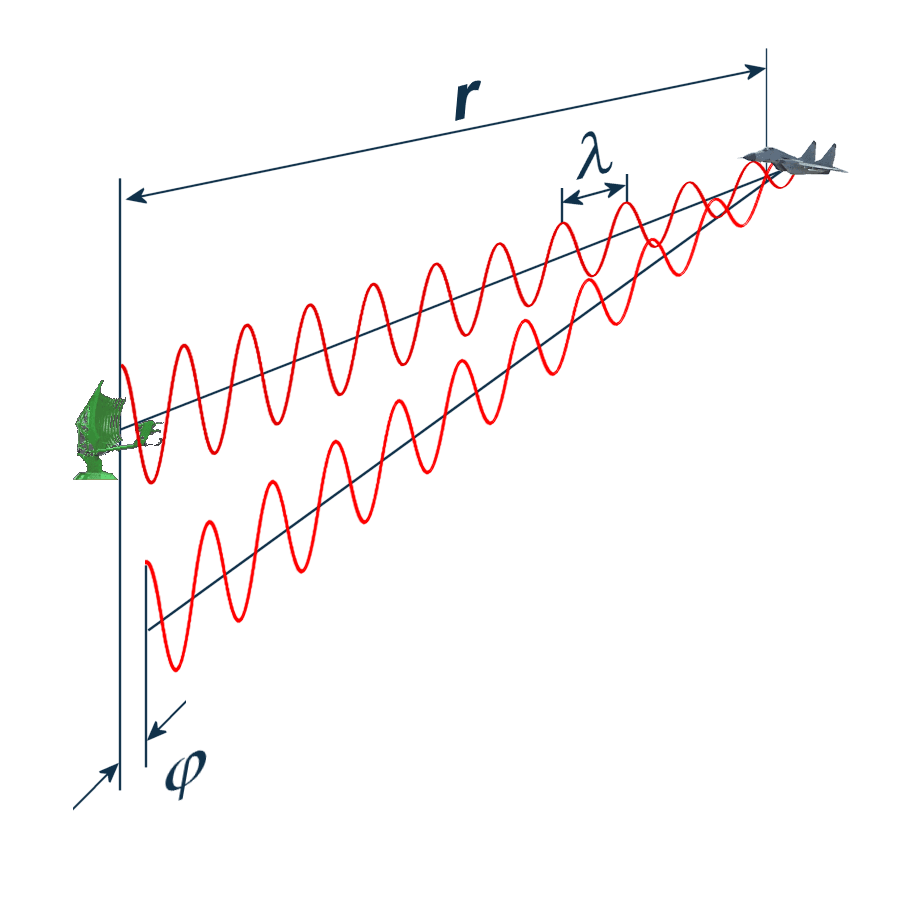
\includegraphics[scale=0.4]{Images/Doppler.png}
\caption{Diagram showing the Doppler shift effect in how an aircraft changes the frequency and that altered frequency is received. Source \cite{Doppler}}
\label{Doppler}
\end{figure}

%---------------------------------------------------------------------------
%	AIRCRAFT EVOLUTION
%---------------------------------------------------------------------------
\section{Aircraft Evolution}
\label{Aircraft Evolution Section}

The early form of aircraft design, was that of a wooden structure to form the skeleton of the aircraft, to which layers of fabrics rolled over this structure powered by a propeller engine to give it thrust. At the time RADAR detection for aircraft was still new and the only detection avoidance that aircraft could obtain is that of visual avoidance. In the 1930s aircraft were made from a light steel structure and aluminium panels to form the fuselage but RADAR was Incorporated heavily and the metal structure of the aircraft allowed the use of the Doppler shift effect to be able to detect aircraft miles away. The design of aircraft focused heavily during World War 2 on speed, survivability and maneuverability, thus RADAR technology overtook the aircraft design by utilizing new higher frequency bandwidths. It was only until the 1960s did the evolution of aircraft take precedent and seek ways to avoid the new radar technology present.

\newpage
\begin{multicols}{2}
\begin{figure}[H]
\centering
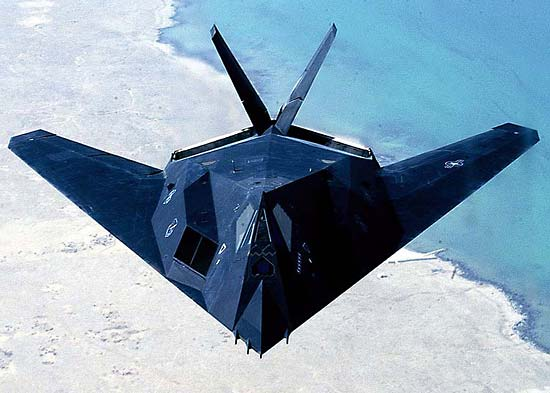
\includegraphics[scale=0.35]{Images/F-117.jpg}
\caption{Figure showing the Lockheed F-117 Nighthawk. Source \cite{F117}}
\label{F117}
\end{figure}

\begin{figure}[H]
\centering
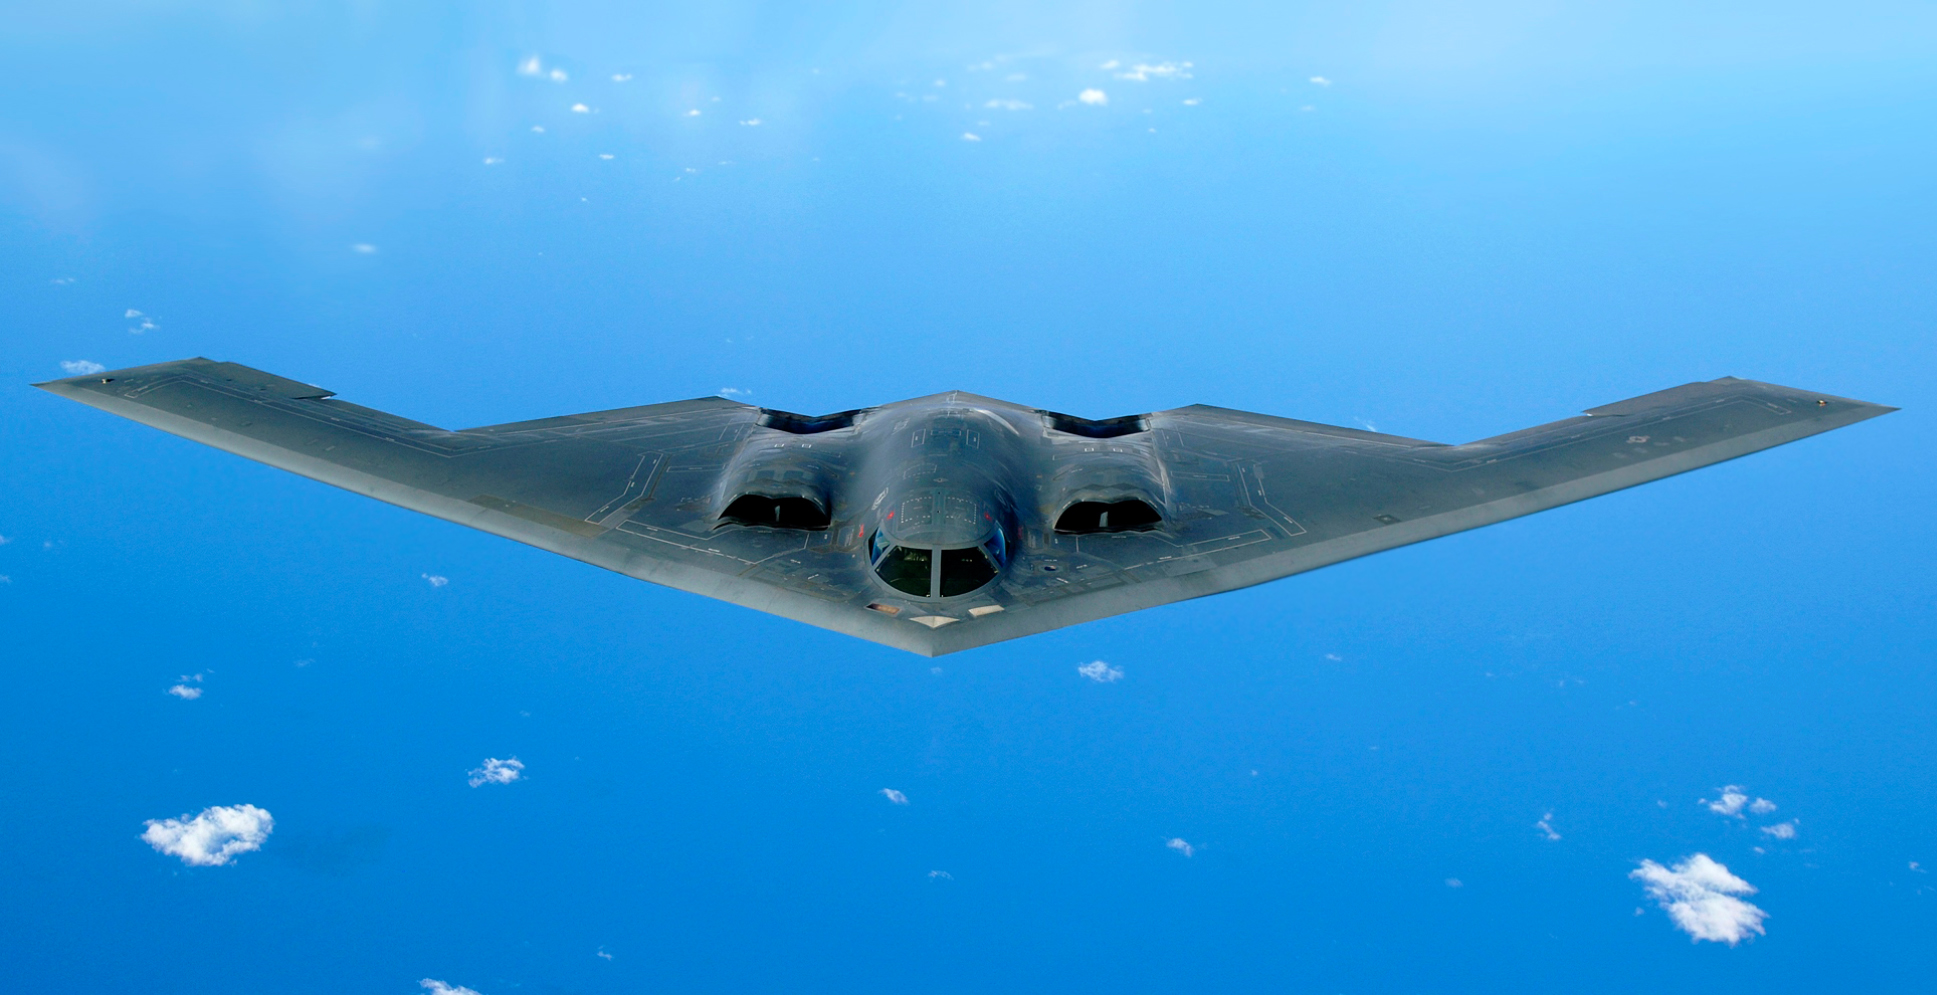
\includegraphics[scale=0.13]{Images/B-2.jpg}
\caption{Figure showing the Northrop Grumman B-2 Spirit. Source \cite{B-2}}
\label{B-2}
\end{figure}
\end{multicols}

The Lockheed F-117 aircraft was designed to be made from radio and electromagnetic wave absorbing materials such as Fibaloy \cite{Ency} as metallic materials were found to reflect the incoming waves better, containing less than 10\% metal. The structure of these both the Lockheed F-117 and Northrop Grumman B-2 Spirit comprised of plastics and carbon-based materials that increase RADAR absorption, the design contains a metallic pyramid structure to shape the aircraft's hull and wings, in between each pyramid section is filled with light absorbing carbon-based materials and sheets of Fibaloy, a absorbent plastic material across this structure \cite{Ency}. This design allowed for the radio/ electromagnetic waves to pass through and bounce through the pyramid structure thus lengthening the waves, this allows for the waves to not be reflected or refracted for detection by the receiver. Though this initial design proved reliant against RADAR detection, further changes were made by covering the engine intakes with metal grids to avoid the signal waves from entering and causing them to be severely distorted and then reflected back to the surface. \\

Furthering the analysis the Northrop Grumman B-2 Spirit "B-2 Stealth Bomber" shown in \cref{B-2} utilising the same absorption methods as the Lockheed F-117 but adapts small right angled cavities in its surface area, this is where when the RADAR signal hits the aircraft the signal catches in these cavities refract the signal instead of reflects them. Though the physical design and makeup of the aircraft changes to avoid detection is that of flying altitude, the Lockheed F-117 was designed to fly low, under the spread of radio and electromagnetic signals, where also flying extremely high also gains detection avoidance as the time of outgoing and incoming RADAR signals is lengthened by the signals journey time. Other key factor is RADAR avoidance is keeping the aircraft cool so that the change in Doppler shift is small, the engines produce vortexes as its pushes the aircraft through the air allowing the Doppler shift to be distorted and refracted back to the receiver. The Lockheed F-117 used no afterburners for this specific reason limiting its speed to subsonic speeds thus used specially for reconnaissance and thus not weapons were held on board making it light and delicate. Ultimately to avoid RADAR detection, to avoid detection aircraft have to be light, slow and have the ability to fly at high altitudes and ultimately in wartime, the aircraft is vulnerable.\\

%---------------------------------------------------------------------------
%	CONCLUSION
%---------------------------------------------------------------------------
\section{Discussion}
\label{Conclusion Section}

In the last century RADAR and aircraft design and technology have both evolved rapidly and reached their physical limitations with current technology. From a simple direct radio wave pulse to an array of highly sensitive radio and electromagnetic waves and the development of LIDAR (Light Imaging Detection and Ranging), RADAR has pushed aircraft to evolve alongside it. Importantly aircraft avoidance (Stealth Technology) was designed and realistically used for militaristic purposes but helped explore, research and discover new materials and understand radio and electromagnetic waves. Though aircraft can be made to be nearly invisible against old and modern RADAR detection methods then aircraft will always be able to be detected even at the smallest level, its also delicate, weak and slow all of which are factors that skirt the laws of flight finely, thus making the materials rare and the cost of the aircraft high. In conclusion a better question to ask would be why do aircraft need to avoid detection if RADAR avoidance is focus in the military sector.  \\

%---------------------------------------------------------------------------
%	REFERENCES
%---------------------------------------------------------------------------
\bibliographystyle{plain}
\bibliography{mybib.bib}
\end{document}